\chapter{Descrizione Autopilota}
In questo capitolo dopo un breve resoconto del sistema su cui è montato l'autopilota, verranno descritte le proprietà dell'hardware e del firmware utilizzato per le simulazioni. Successivamente gli strumenti messi a disposizione per la code-generation e le simulazioni e come sono stati utilizzati per ricavare i risultati finali.

\section{Descrizione del hardware}

Il drone considerato durante le simulazioni è un quadrirotore composto da una struttura centrale fatta di alluminio e fibra di carbonio. Su questa struttura sono montati i motori brushless con le pale e le rispettiva protezioni. Vi sono inoltre posizionati l'autopilota CUAV\textregistered V5 Nano\textregistered, modello aggiornato rispetto alla precedente configurazione utilizzante PixHawk 2.1 Cube e Rasperry Pi 3B, \cite{DesTestCarm}.

In figura (\ref{fig:DRONE}), viene mostrata una foto indicativa del drone dove verrà posizionato l'autopilota. Nella tabella (\ref{tab:DRONE}), vengono riportati i parametri principali di questa configurazione, valutati attraverso una stima fatta da un modello CAD, \cite{DesTestCarm}.

\begin{figure}
	\centering
	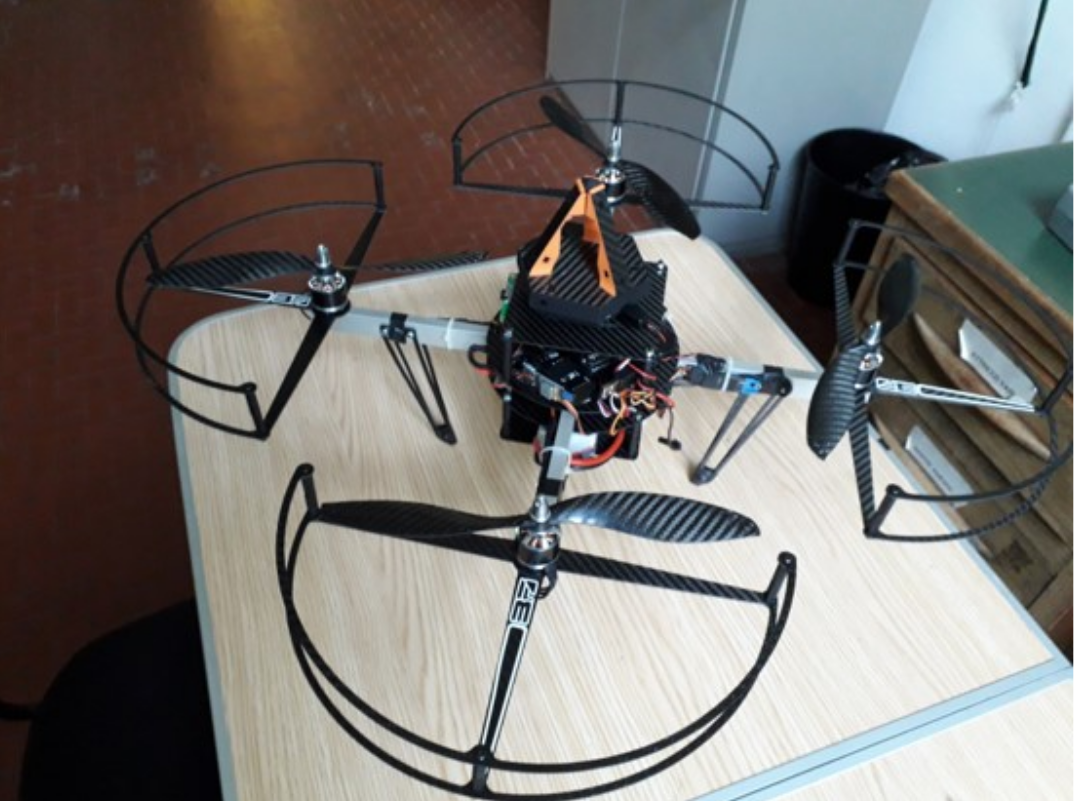
\includegraphics[width=0.7\textwidth]{DescrizioneAutopilota/Figure/DRONE}
	\caption{Prototipo di riferimento}
	\label{fig:DRONE}
\end{figure}

\begin{table}
	\centering
	\begin{tabular}{c c}
		\hline
		Massa $m$ & 1.5 [kg] \\
		Inerzia $J_x$ & 0.0170 [$\text{kgm}^2$] \\
		Inerzia $J_y$ & 0.0173 [$\text{kgm}^2$] \\
		Inerzia $J_z$ & 0.0308 [$\text{kgm}^2$] \\
		Diametro pala & 10 [in]\\
		\hline
	\end{tabular}	
	\caption{Principali caratteristiche del drone}
	\label{tab:DRONE}
\end{table}

Come accennato l'autopilota per la quale avverrà la code-generation dei modelli di controllo è un CUAV\textregistered V5 Nano\textregistered, mostrato in Figura (\ref{fig:CUAV}).

\begin{figure}
	\centering
	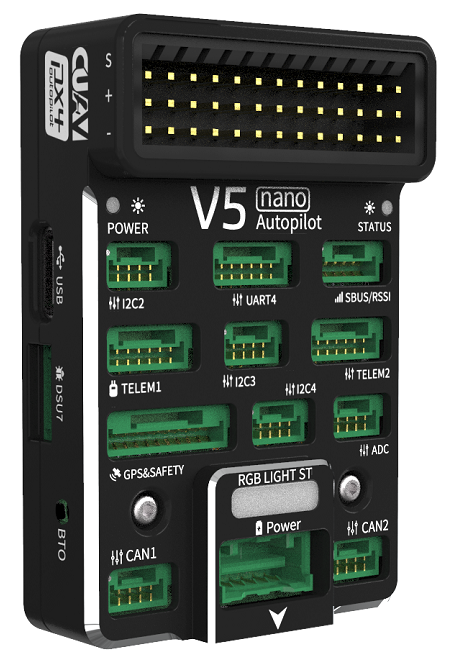
\includegraphics[width=0.4\textwidth]{DescrizioneAutopilota/Figure/CUAV}
	\caption{CUAV\textregistered V5 Nano , \cite{CUAV}}
	\label{fig:CUAV}
\end{figure}

Questo autopilota è stato progettato da CUAV\textregistered in collaborazione con il team di sviluppo del firmware PX4, \cite{CUAV}. L'autopilotta è miniaturizzato ed è progettato per applicazioni indoor, integrando alcuni sensori al suo interno.
Vengonho ora elencate le caratteristiche fondamentali e i componenti.
\begin{itemize}
	\item \textbf{Processore:} STM32F765 32 Bit Arm\textregistered Cortex\textregistered-M7, 216MHz, 2MB di memoria, 512KB RAM
	\item \textbf{Sensori integrati:} 
		\begin{itemize}
			\item Accelerometro/Giroscopio: ICM-20689
			\item Accelerometro/Giroscopio: ICM-20602
			\item Accelerometro/Giroscopio: BMI055
			\item Magnetometro: IST8310
			\item Barometro: MS5611
		\end{itemize}
	\item \textbf{Canali d input/output:}
		\begin{itemize}
			\item 8 uscite PWM
			\item 3 uscite PWM/ingressi per la Flight Management Unit (FMU)
			\item porta dedicata all'input del Radio Control (R/C) utilizzando la Combined Pulse Position Modulation (CPPM)
			\item porta dedicata all'input del Radio Control (R/C) utilizzando protocollo Spektrum / DSM e S.Bus
			\item porta analogica / input Received Rignal Rtrength Rndicator (RSSI) per la PWM
			\item 4 porte seriali di utilizzo generico
			\item 3 porte Inter-Integrated Circuit (I2C)
			\item 4 canali Serial Peripheral Interface (SPI) 
			\item 2 canali Controller Area Network (CAN)
			\item ingresso per la batteria
			\item 2 ingressi analogici aggiuntivi
			\item supporto per tecnologia nARMED
		\end{itemize}
	\item \textbf{Alimentazione da batteria:} 4.75 - 5.5 V
	\item \textbf{Alimentazione da Universal Serial Bus (USB):} 4.75 - 5.25 V
	\item \textbf{Dimensioni:} 60*40*14 mm
	\item \textbf{Temperatura operativa:} -20 - 80 °C

\end{itemize}



